\icode{N25Y-MM-SI-L3-261011-001}
\nceeID[4]{2025广东}{7}
如图所示，在光滑的水平面上，小球\(M\)、\(N\)分别在水平恒力\(F_1\)、\(F_2\)作用下，由静止开始在同一直线相向运动，在\(t_1\)时刻发生正碰后各自反向运动。已知\(F_1\)和\(F_2\)始终大小相等、方向相反，从开始运动到碰撞后速度第1次减为0过程中，两小球速度\(v\)随时间\(t\)变化的图像，可能正确的是\paren[]

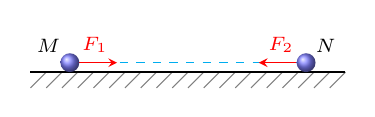
\begin{tikzpicture}[font=\scriptsize]
	\foreach \x in{0,.2,...,3.8}
		\draw[gray] (\x,-.2)--++(.2,.2);
	\draw[thick] (0,0)--(4,0);
	\draw[dashed,cyan] (.5,.12)coordinate(a)--(3.5,.12)coordinate(b);
	\draw[red,-stealth] (a)--++(.6,0)node[above left]{\(F_1\)};
	\draw[red,-stealth] (b)--++(-.6,0)node[above right]{\(F_2\)};
	\shade[ball color=blue!50] (a)node[above left]{\(M\)} circle(.12);
	\shade[ball color=blue!50] (b)node[above right]{\(N\)} circle(.12);
\end{tikzpicture}

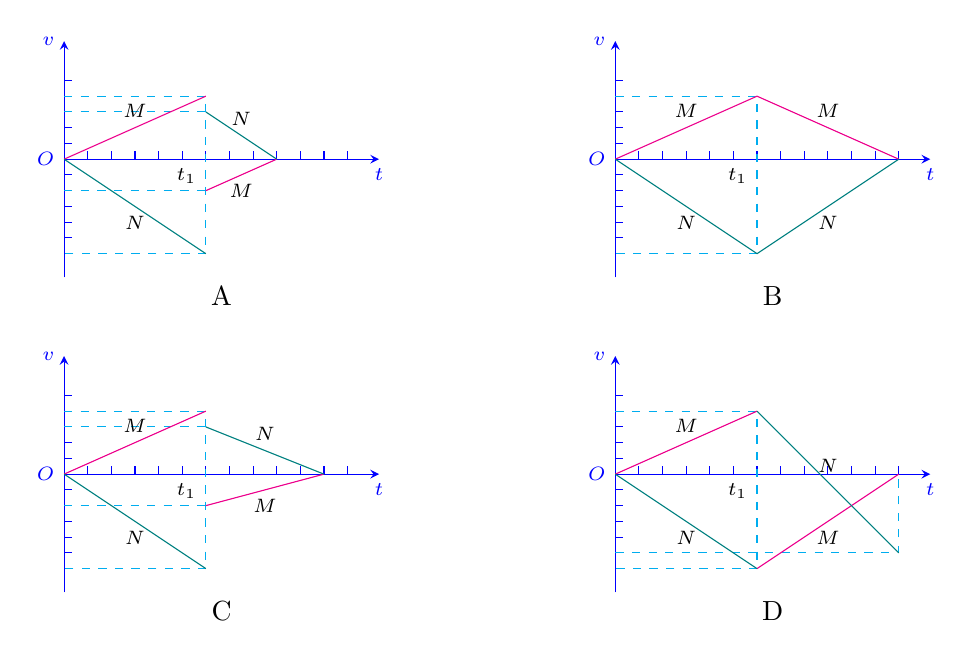
\begin{tikzpicture}[>=stealth,font=\scriptsize]
	\begin{scope}
		\node at(2,-1.5)[below,font=\normalsize]{A};
		\foreach \x in{.3,.6,...,3.9}
			\draw[blue] (\x,0)--++(0,.1);
		\draw[blue,->] (0,0)node[left]{\(O\)}--(4,0)node[below]{\(t\)};
		\foreach \y in{-1.2,-1,...,1}
			\draw[blue] (0,\y)--++(.1,0);
		\draw[blue,->] (0,-1.5)--(0,1.5)node[left]{\(v\)};
		\node at(1.8,0)[below left]{\(t_1\)};
		\draw[dashed,cyan] (0,.8)--(1.8,.8)--(1.8,-1.2)--(0,-1.2) (0,.6)--(1.8,.6) (0,-.4)--(1.8,-.4);
		\draw[magenta] (0,0)--node[above,black]{\(M\)}(1.8,.8) (1.8,-.4)--node[below,black]{\(M\)}(2.7,0);
		\draw[teal] (1.8,.6)--node[above,black]{\(N\)}(2.7,0) (0,0)--node[below,black]{\(N\)}(1.8,-1.2);
	\end{scope}
	\begin{scope}[xshift=7cm]
		\node at(2,-1.5)[below,font=\normalsize]{B};
		\foreach \x in{.3,.6,...,3.9}
			\draw[blue] (\x,0)--++(0,.1);
		\draw[blue,->] (0,0)node[left]{\(O\)}--(4,0)node[below]{\(t\)};
		\foreach \y in{-1.2,-1,...,1}
			\draw[blue] (0,\y)--++(.1,0);
		\draw[blue,->] (0,-1.5)--(0,1.5)node[left]{\(v\)};
		\node at(1.8,0)[below left]{\(t_1\)};
		\draw[dashed,cyan] (0,.8)--(1.8,.8)--(1.8,-1.2)--(0,-1.2);
		\draw[magenta] (0,0)--node[above,black]{\(M\)}(1.8,.8) (1.8,.8)--node[above,black]{\(M\)}(3.6,0);
		\draw[teal] (0,0)--node[below,black]{\(N\)}(1.8,-1.2) (1.8,-1.2)--node[below,black]{\(N\)}(3.6,0);
	\end{scope}
	\begin{scope}[yshift=-4cm]
		\node at(2,-1.5)[below,font=\normalsize]{C};
		\foreach \x in{.3,.6,...,3.9}
			\draw[blue] (\x,0)--++(0,.1);
		\draw[blue,->] (0,0)node[left]{\(O\)}--(4,0)node[below]{\(t\)};
		\foreach \y in{-1.2,-1,...,1}
			\draw[blue] (0,\y)--++(.1,0);
		\draw[blue,->] (0,-1.5)--(0,1.5)node[left]{\(v\)};
		\node at(1.8,0)[below left]{\(t_1\)};
		\draw[dashed,cyan] (0,.8)--(1.8,.8)--(1.8,-1.2)--(0,-1.2) (0,.6)--(1.8,.6) (0,-.4)--(1.8,-.4);
		\draw[magenta] (0,0)--node[above,black]{\(M\)}(1.8,.8) (1.8,-.4)--node[below,black]{\(M\)}(3.3,0);
		\draw[teal] (1.8,.6)--node[above,black]{\(N\)}(3.3,0) (0,0)--node[below,black]{\(N\)}(1.8,-1.2);
	\end{scope}
	\begin{scope}[yshift=-4cm,xshift=7cm]
		\node at(2,-1.5)[below,font=\normalsize]{D};
		\foreach \x in{.3,.6,...,3.9}
			\draw[blue] (\x,0)--++(0,.1);
		\draw[blue,->] (0,0)node[left]{\(O\)}--(4,0)node[below]{\(t\)};
		\foreach \y in{-1.2,-1,...,1}
			\draw[blue] (0,\y)--++(.1,0);
		\draw[blue,->] (0,-1.5)--(0,1.5)node[left]{\(v\)};
		\node at(1.8,0)[below left]{\(t_1\)};
		\draw[dashed,cyan] (0,.8)--(1.8,.8)--(1.8,-1.2)--(0,-1.2) (0,-1)--(3.6,-1)--(3.6,0);
		\draw[magenta] (0,0)--node[above,black]{\(M\)}(1.8,.8) (1.8,-1.2)--node[below,black]{\(M\)}(3.6,0);
		\draw[teal] (1.8,.8)--node[above,black]{\(N\)}(3.6,-1) (0,0)--node[below,black]{\(N\)}(1.8,-1.2);
	\end{scope}
\end{tikzpicture}
\begin{answer}
    A\qquad 提示：碰撞动量守恒
\end{answer}